% Author: Izaak Neutelings (March 2020)
\documentclass[border=3pt,tikz]{standalone}
\usepackage{amsmath} % for \dfrac
\usepackage{physics}
\usepackage{tikz,pgfplots}
\usepackage{tikz-3dplot}
\usepackage[outline]{contour} % glow around text
\usetikzlibrary{angles,quotes} % for pic (angle labels)
\usetikzlibrary{arrows,arrows.meta}
\usetikzlibrary{calc}
\usetikzlibrary{decorations.markings}
\tikzset{>=latex} % for LaTeX arrow head
\usepackage{xcolor}
\colorlet{veccol}{green!45!black}
\colorlet{Bcol}{violet!90}
\colorlet{BFcol}{red!70!black}
\colorlet{veccol}{green!45!black}
\colorlet{Icol}{blue!70!black}
\colorlet{Ampcol}{green!60!black!70}
\tikzstyle{BField}=[->,thick,Bcol]
\tikzstyle{current}=[->,Icol,thick]
\tikzstyle{force}=[->,thick,BFcol]
\tikzstyle{vector}=[->,thick,veccol]
\tikzstyle{velocity}=[->,very thick,vcol]
\tikzstyle{charge+}=[very thin,draw=black,top color=red!50,bottom color=red!90!black,shading angle=20,circle,inner sep=0.5]
\tikzstyle{charge-}=[very thin,draw=black,top color=blue!50,bottom color=blue!80,shading angle=20,circle,inner sep=0.5]
\tikzstyle{metal}=[line width=0.3,top color=black!15,bottom color=black!25,middle color=black!20,shading angle=10]
\tikzstyle{darkmetal}=[line width=0.4,top color=red!20!black!40,bottom color=red!20!black!70,middle color=red!20!black!30,shading angle=10]
\tikzstyle{measline}=[{Latex[length=3]}-{Latex[length=3]}]
\tikzset{
  BFieldLine/.style={thick,Bcol,decoration={markings,mark=at position #1 with {\arrow{latex}}},
                                 postaction={decorate}},
  BFieldLine/.default=0.5,
  Ampcurve/.style={thick,Ampcol,decoration={markings,mark=at position #1 with {\arrow{latex}}},
                                postaction={decorate}},
  Ampcurve/.default=0.55,
  pics/Bin/.style={
    code={
      \def\R{0.12}
      \draw[pic actions,line width=0.6,#1,fill=white] % ,thick
        (0,0) circle (\R) (-135:.75*\R) -- (45:.75*\R) (-45:.75*\R) -- (135:.75*\R);
  }},
  pics/Bout/.style={
    code={
      \def\R{0.12}
      \draw[pic actions,line width=0.6,#1,fill=white] (0,0) circle (\R);
      \fill[pic actions,#1] (0,0) circle (0.3*\R);
  }},
  pics/Bin/.default=Bcol,
  pics/Bout/.default=Bcol,
}
\tikzstyle{measure}=[fill=white,midway,outer sep=2]
\contourlength{1.4pt}

% RING SHADING
\makeatletter
\pgfdeclareradialshading[tikz@ball]{ring}{\pgfpoint{0cm}{0cm}}%
{rgb(0cm)=(1,1,1);
rgb(0.719cm)=(1,1,1);
color(0.72cm)=(tikz@ball);
rgb(0.9cm)=(1,1,1)}
\tikzoption{ring color}{\pgfutil@colorlet{tikz@ball}{#1}\def\tikz@shading{ring}\tikz@addmode{\tikz@mode@shadetrue}}
\makeatother


\begin{document}


% WIRE MAGNETIC FIELD VERTICAL
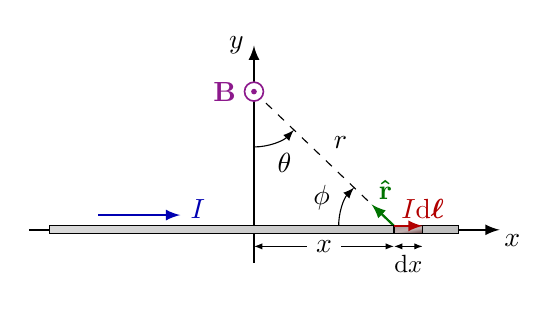
\begin{tikzpicture}
  \def\L{5.2}
  \def\W{0.10}
  \def\xmin{-0.55*\L}
  \def\xmax{0.6*\L}
  \def\ymin{-0.08*\L}
  \def\ymax{0.45*\L}
  \def\x{0.342*\L}
  \def\dx{0.07*\L}
  \coordinate (O) at (0,0);
  \coordinate (P) at (0,0.75*\ymax);
  \coordinate (X) at (\x,\W/2);
  
  % AXIS
  \draw[->,thick] (\xmin,0) -- (\xmax,0) node[below right=-2] {$x$};
  \draw[->,thick] (0,\ymin) -- (0,\ymax) node[left] {$y$};
  
  % MEASURES
  %\draw[<->] (0,0.2*\ymax) --++ (\x,0) node[midway,above] {$x$};
  \draw[measline] (    0,-0.09*\ymax) --++ (\x,0) node[measure] {$x$};
  \draw[measline] (   \x,-0.09*\ymax) --++ (\dx,0) node[midway,below,scale=0.9] {$\dd{x}$};
  %\draw[measline] (-\L/2,0.65*\ymin) --++ (\L,0) node[measure,right=10] {$L$};
  
  % POINT
  \node[Bcol,left=3] at (P) {$\vb{B}$};
  \draw[dashed] (P) -- (X) node[midway,above right] {$r$};
  \draw pic[->,"$\theta$",draw=black,angle radius=20,angle eccentricity=1.4] {angle = O--P--X};
  \draw pic[<-,"$\phi$",draw=black,angle radius=20,angle eccentricity=1.4] {angle = P--X--O};
  \draw[vector] (X) -- ($(X)!0.16!(P)$) node[right=5,above=-2] {$\vu{r}$};
  
  % VECTORS
  \draw[current] (-0.38*\L,0.08*\ymax) --++ (0.2*\L,0) node[above=2,right] {$I$};
  \pic at (P) {Bout}; %={fill=white}
  
  % ROD
  \draw[metal] (-\L/2,-\W/2) rectangle ++(\L,\W);
  \draw[darkmetal] (\x,-\W/2) rectangle ++(\dx,\W);
  %  node[midway,right=10,above=3] {$I\dd{x}$}; %I\dd{\ell}=
  \draw[force]
    (X) --++ (\dx,0) node[above=-1] {$I\!\dd{\vb*{\ell}}$};
  
\end{tikzpicture}


% WIRE MAGNETIC FIELD angles
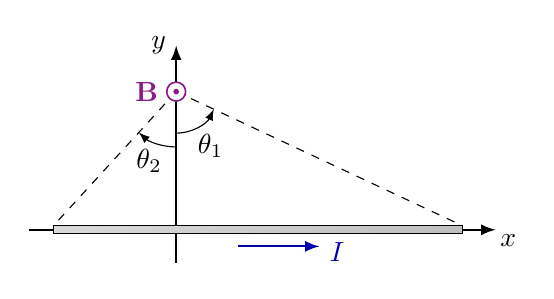
\begin{tikzpicture}
  \def\L{5.2}
  \def\W{0.10}
  \def\shift{0.6}
  \def\xmax{0.6*\L}
  \def\ymin{-0.08*\L}
  \def\ymax{0.45*\L}
  \def\x{0.342*\L}
  \def\dx{0.07*\L}
  \coordinate (O) at (0,0);
  \coordinate (P) at (0,0.75*\ymax);
  \coordinate (L) at (-\shift*\L/2,\W/2);
  \coordinate (R) at ({(1-\shift/2)*\L},\W/2);
  
  % AXIS
  \draw[->,thick] (-\shift*\xmax,0) -- ({(0.7+\shift)*\xmax},0) node[below right=-2] {$x$};
  \draw[->,thick] (0,\ymin) -- (0,\ymax) node[left] {$y$};
  
  % POINT
  \node[Bcol,left=3] at (P) {$\vb{B}$};
  \draw[dashed] (P) -- (L); %node[midway,above right] {$r$};
  \draw[dashed] (P) -- (R); %node[midway,above right] {$r$};
  \draw pic[<-,"$\theta_2$",draw=black,angle radius=20,angle eccentricity=1.35] {angle = L--P--O};
  \draw pic[->,"$\theta_1$",draw=black,angle radius=15,angle eccentricity=1.55] {angle = O--P--R};
  
  % VECTORS
  \draw[current] (0.15*\L,-0.09*\ymax) --++ (0.2*\L,0) node[below=2,right] {$I$};
  \pic at (P) {Bout}; %={fill=white}
  \draw[metal] (-\shift*\L/2,-\W/2) rectangle ++(\L,\W);
  
\end{tikzpicture}


% WIRE B FIELD 3D
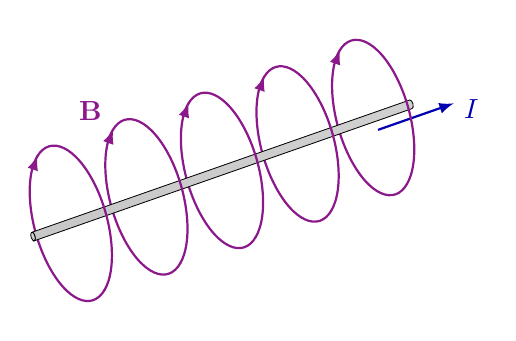
\begin{tikzpicture}[z={(0.8,0.28)},x={(0.58,-0.45)}]
  \def\L{6}
  \def\W{0.10}
  \def\R{0.9}
  \def\ang{-35}
  \def\scale{1.3}
  \def\NB{5}
  \coordinate (O) at (0,0,0);
  %\draw (0,0,0) -- (2,0,0);
  %\draw (0,0,0) -- (0,0,2);
  
  % B FIELD BACK
  \foreach \i [evaluate={\x=(\i-\NB/2-0.5)*\L/\NB;}] in {1,...,\NB}{
    %\draw[BField,-] (0,0,\x)++(\ang+1:\R) arc (\ang+1:\ang-181:\R);
    \draw[BFieldLine=1] (0,0,\x)++(\ang+1:\R) arc (\ang+1:\ang-181:\R) --++ (65:0.001*\R);
  }
  
  % WIRE
  \draw[metal] (0,0,-\L/2)++(120:\W/2) --++ (0,0,\L) arc (120:-60:\W/2) --++ (0,0,-\L) arc (-60:120:\W/2);
  \draw[metal] (0,0,-\L/2) circle (\W/2);
  \draw[current] (0.12*\R,-0.12*\R,0.4*\L) --++ (0,0,0.2*\L) node[below=2,right] {$I$};
  
  % B FIELD FRONT
  \foreach \i [evaluate={\x=(\i-\NB/2-0.5)*\L/\NB;}] in {1,...,\NB}{
    %\draw[BFieldLine=1] (0,0,\x)++(\ang+180:\R) arc (\ang+180:\ang:\R) --++ (-116:0.001*\R);
    \draw[BField,-] (0,0,\x)++(\ang+180:\R) arc (\ang+180:\ang:\R);
  }
  \node[Bcol] at (-0.9*\R,0.9*\R,-0.25*\L) {$\vb{B}$}; %++(140:1.3*\R)
  
\end{tikzpicture}


% WIRE MAGNETIC FIELD + Ampere's loop
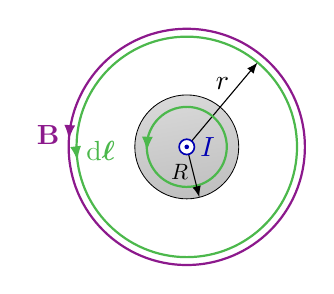
\begin{tikzpicture}
  \def\R{0.66}
  \def\RB{1.5}
  \def\RA{1.4}
  \def\RAin{0.77*\R}
  \def\NB{2}
  
  % AXIS
  \draw[metal] (0,0) circle (\R);
  \draw[->] (0,0) -- (50:\RA) node[midway,right=8,above left=2] {$r$};
  
  % AMPERE LOOP
  \draw[Ampcurve={0.52}] (0,0) circle (\RA);
  \draw[Ampcurve={1}] (-175:\RAin) arc (-175:185:\RAin) --++ (-92:0.01);
  \node[Ampcol,right] at (182:\RA) {$\dd\vb*{\ell}$};
  
  % CURRENT
  \draw[->] (0,0) -- (-76:\R) node[midway,left=-1,scale=0.8] {$R$};
  \pic[scale=0.81] at (0,0) {Bout={Icol}};
  \node[Icol] at (0:0.4*\R) {$I$};
  
  % MAGNETIC FIELDLINES
  %\foreach \i [evaluate={\r=\RB*\i)}] in {1,...,\NB}{
  \draw[BFieldLine={0.49}] (0,0) circle (\RB);
  %}
  \node[Bcol,left] at (174:\RB) {$\vb{B}$};
  
\end{tikzpicture}


\end{document}
